

\chapter{Introduction}
\lettrine{V}{ision} based relative navigation is becoming increasingly important to enable the development of next-generation space missions, such as the exploration of natural celestial bodies, On Orbit Servicing (OOS), Formation Flying (FF) or Active Debris Removal (ADR). In this context, the necessity of real-time guidance and decision making in a dynamical environment makes onboard relative attitude and position estimation paramount for the successful completion of the mission objectives. \\
 Within the previously mentioned mission scenarios, ADR has recently gained significant interest because of the growing concern about space situational awareness. Dealing with inherently non-cooperative targets, ADR mission shall be equipped with vision-based sensors able to provide a high-frequency relative pose estimation so to avoid undesired collisions with the target.\\
%\lettrine{W}{ith} the ever-increasing number of uncooperative artificial objects in orbital regions such as LEO and GEO and the risk associated with their presence, the necessity for mitigation strategies such as Active Debris Removal (ADR) has become even more urgent in recent years. Because of the fast dynamics when performing close proximity operations about an uncooperative target, ADR missions face very challenging conditions for the GNC subsystem. To avoid undesired collisions, it is paramount to estimate onboard the relative position and attitude with respect to the target. \\ 
In this context, monocular cameras in the visible spectrum present a very mass and power-effective solution, although presenting important operational limitations. Their strong dependency on the illumination conditions of the target limits their range of applications in case of low illumination conditions or eclipse. A promising solution to enhance the reliability of monocular cameras is to use collaboratively two sensors working in the visible and thermal spectrum. Thermal imaging sensors measure the thermal radiance of the target, which is influenced by the illumination coming from the Sun, but it is not subject to shadowing or reflections. However, the overall quality provided by thermal imaging sensors is lower because the images produced are subject to a higher blur and a lower resolution. \\
%Thermal imaging sensors provide lower-quality data in terms of blur and image resolution but are independent of illumination conditions as they measure the thermal radiance of the target.\\
In this framework, the thesis proposes a novel navigation pipeline that exploits an Extended Kalman Filter to perform feature-level adaptive sensor fusion between the two cameras. The stand-alone vision-based navigation chain is tested on synthetically generated images to assess its performances, evaluating as well the capability to perform TIR-only navigation in low illumination conditions. \\
The present chapter further details the motivation for the thesis work and presents the literature related to the investigated subject. Finally, the work's intended contribution is presented with a general overview and the thesis outline.

\section{Context \& motivation}
\label{sec:contandmotiv}
\chaptermark{Introduction}
\subsection{Active Debris Removal}
Since the beginning of spaceflight, the amount of artificial objects in orbit has increased steadily. In particular, non-cooperative objects, better known as space debris, threaten satellites operating in certain orbital families such as Low Earth Orbits. 
Awareness of this problem led to the publication in 2002 of the IADC Space Debris Mitigation Guidelines \cite{yakovlev2005iadc} by the InterAgency Debris Coordination Committee, superseded by the 2011 ISO standard 24113 \cite{ISO24113} on debris mitigation requirements. These standards have been adopted by the European Committee for Space Standardization (ECSS) and apply to all projects developed by the European Space Agency (ESA).\\
However, the effect that such recommendations have had is limited. Firstly, entities operating space missions are not required to follow them, as they are not applicable regulations.
Furthermore, even if these were strictly followed, the environment is unstable \cite{lemmens2020esa}, i.e., the number of debris will increase even if all space activities are interrupted because of consecutive impacts of existing objects. An identified solution to limit the growth of the number of space debris is to actively deorbit human-made objects with ADR missions. According to \cite{liou2012active}, removing five Intact Derelict Objects (IDOs) per year would stabilize the situation in LEO. IDOs comprises mainly inoperative satellites, such as the European debris ENVISAT, launcher stages and payload adapters.\\
ADR missions aim at interacting with space objects to reduce their orbital lifetime. In this context, the active spacecraft is referred to as chaser, while the spacecraft to be decommissioned is the target. The mission profile of an ADR mission can be subdivided into different operational phases, presented in \cref{fig:phases}. After being launched, the chaser phases with the target orbit reaching an hold point, relying on absolute navigation. Subsequently, during the inspection phase, the chaser collects information about the target with onboard sensors to plan the subsequent phases. The duration of this phase and the distance maintained from the target depends on the prior knowledge about the target, and the characteristics of the sensors of the chaser. For the inspection, it is necessary to rely also on relative navigation, as the shorter the chaser-target distance, the higher the risk of collision. The information collected during the inspection phase is confirmed and improved during the fly-around phase, further approaching the target. Once gathered the required information the chaser performs the final approach and capture in order to capture the target. Finally, the target is safely disposed in the stabilization and de-orbiting phase.\\
The first mission to perform this task will be the ClearSpace-1 mission in 2025 \cite{biesbroek2021clearspace}, commissioned by ESA. The mission aims to deorbit VEga Secondary Payload Adapter (VESPA). \\

\begin{figure}[!h]
    \centering
    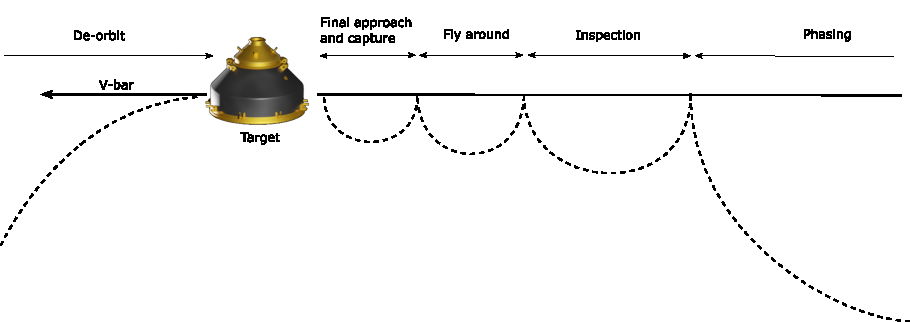
\includegraphics[width = \linewidth]{Images/phases.pdf}
    \caption{Simplified schematic of the typical phases of an ADR mission}
    \label{fig:phases}
\end{figure}

\subsection{Autonomous visual navigation}
\chaptermark{Introduction}
For applications including Close-Proximity Operations (CPO) and Active Debris Removal, it is paramount to have a high degree of onboard autonomy. To avoid the risk of an undesired contact with the target, the chaser shall be able to operate autonomously to be robust against communication delays or unavailability. In this framework, the necessity to have continuous relative position and attitude estimation with respect to the target is evident. \\
Unlike Formation Flying or In-Orbit Assembly scenarios, in the case of navigation around space debris, the target is always non-cooperative. Therefore, visual navigation must be used to estimate the relative position and attitude, using optical sensors such as Light Detection and Ranging (LiDAR), stereo cameras, or monocular cameras. For the selection of the navigation sensor, its precision and range of applicability are paramount. However, the trade-off shall consider parameters like mass, power consumption, the processing power required, and cost. Monocular cameras represent a more mass and power-effective solution than LiDAR while granting a more comprehensive operational range than stereo cameras  \cite{pesce2019autonomous,piccinin2023spacecraft}. \\
The Orbital Express carried out the first in flight-demonstration of autonomous docking to a non-cooperative spacecraft in 2007 \cite{pinson2008orbital}, commissioned by DARPA, using optical images and a system of corner-cube reflectors. Additional flight heritage is given by the PRISMA mission in 2010 \cite{karlsson2014prisma}, providing a more relevant example of the usage of monocular cameras. The mission was composed of two spacecrafts: Mango and Tango. The Vision Based Sensor mounted on Mango comprised two monocular cameras, one for far range and one for close range operations, working in the visible spectrum. Within the multiple mission objectives, Mango performed an autonomous vision-based rendezvous with Tango acting like a non-cooperative target. Once this was completed, an additional experiment, IRIDES, was added to test the visual navigation pipeline to rendezvous and inspect the uncooperative Picard spacecraft. However, the rendezvous could not be tested because of the delta-v depletion before the phasing with Picard \cite{doi:10.2514/1.G003239}. Finally, to consolidate the results of the PRISMA mission, the German Aerospace Center (DLR) launched the Autonomous Vision Approach Navigation and Target Identification (AVANTI) experiment onboard the BRIOS spacecraft \cite{gaias2018flight}, aimed at demonstrating autonomous rendezvous from $\SI{10}{\kilo\meter}$ to $\SI{1}{\kilo\meter}$ towards an uncooperative spacecraft making use of visual angles-only measurements. To achieve this result, the same far-range navigation camera as PRISMA was mounted on BRIOS.\\
Despite the significant progress made in the last decades and the flight heritage given by past missions, navigation technologies for autonomous relative navigation about uncooperative targets still require further development to de-risk them and increase their robustness. Moreover, the development of more reliable navigation solutions for the ADR application would have a positive effect on other mission scenarios. The increased interest in missions involving OOS and FF requires improving the current state of the art of navigation technologies. A planned mission aimed at contributing to this aspect is the ESA mission e.Inspector, which includes within its mission objectives to test optical technologies for navigation about an uncooperative target. Within the proposed architecture to be mounted onboard e.Inspector, currently in phase B of its development, it is proposed a combination of visible and thermal monocular cameras. The addition of the thermal camera serves to increase the range of applications of the visible one to different illumination conditions. 
%As an identified shortfall of visible monocular cameras is the high dependency on illumination conditions, a promising solution is using cameras working in multiple spectra, such as long-wave infrared (LWIR). 


\subsection{Thermal imaging}
Because of their wide range of applications and long history of use, cameras working in the visible spectrum (VIS) provide high-quality data with low power consumption. This is not the case for thermal (TIR) cameras. TIR cameras based on cooled microbolometers, working in the Mid-Wave ($\SI{3}{\micro\meter}$ - $\SI{8}{\micro\meter}$) to Long-Wave ($\SI{8}{\micro\meter}$ - $\SI{15}{\micro\meter}$) infrared, are not suitable for space applications due to the power required and the complexity of the cryogenic cooling of the bolometer. The state of the art for space scenarios consists of uncooled sensors working only in the Long-Wave infrared, providing sufficient sensitivity without the issues of cooling the sensor \cite{cassinis2019review}. 
The flight heritage of this sensor is relatively limited, as it was tested only on the LIRIS experiment onboard the ATV5 Mission \cite{cavrois2015liris} and later on the Raven ISS Hosted Payload \cite{galante2016fast}. \\
% Add asteroid navigation
Additional heritage is provided in the context of asteroid exploration. The Hayabusa 2 mission \cite{okada2017thermal} acquired close range thermal images of the Ryugu asteroid in the Long Wave InfraRed spectrum. The thermal imaging was not performed for the purpose of relative navigation, although it was noted that in the thermal spectrum it was possible to clearly identify  visual markers placed on the surface as cold spots, highlighting the possibility of multispectral navigation. This technology will be tested  for asteroid navigation in the ESA mission Hera \cite{michel2022esa}, mounting the TIRI (Thermal InfraRed Imager) payload provided by JAXA (Japan Aerospace Exploration Agency). \\
Compared to VIS cameras, TIR sensors are less sensitive to different illumination conditions because they depend on the thermal profile of the target and its emitted radiation. Thus, the thermal cameras could be employed also when the target is not illuminated if its temperature is within the sensor's sensibility ranges. However, the image resolution is lower than VIS cameras, with a higher blur that reduces its performance for relative navigation. 
Because of the limitations of both visible and thermal imaging sensors, combining the two represents a promising solution for increasing the robustness of relative optical navigation.

\section{Literature review}
\chaptermark{Introduction}
This section presents the current state of the art in multispectral visual navigation. The literature is reviewed with a top-down approach, beginning with an overview of monocular pose estimation methods, followed by a discussion of common filtering approaches for relative navigation, and concluding with an examination of the latest developments in multispectral data fusion for navigation applications.

\subsection{Monocular pose estimation}
Monocular pose estimation is the process estimating a target spacecraft's relative attitude and position with respect to a chaser spacecraft, using the measurements output of a single monocular camera or multiple cameras fused together. \\
The taxonomy of pose estimation methods divides them based on how the image information is exploited. In appearance-based approaches, also known as direct methods, the raw visual measurement in terms of pixels is used \cite{mohamed2019survey}. Algorithms such as the Active Appearance Model (AAM) or the Principal Component Analysis (PCA) are used to match the object detected in the image to a stored database of the target images. This approach, although often implemented in robotics and surveillance applications, is less suitable for space applications because of its scarce robustness to noise in the images or elements in the background, which are common elements of space imagery \cite{cassinis2019review,opromolla2017review}.\\
More suitable approaches for space applications are the feature based-methods, which exploit relevant features of the image, such as corners or edges, to reconstruct the target's pose. These methods apply to navigation about both known and unknown targets. If the shape of the target is not known, a common solution is to reconstruct it with the available measurements. This is commonly accomplished with Simultaneous Localization and Mapping (SLAM) \cite{durrant2006simultaneous}, a real-time process where the chaser computes at the same time its location (Localization) and a map of the target (Mapping). As the navigation about unknown objects is outside the thesis work, the reader is referred to \cite{opromolla2017review} for a broad overview of uncooperative pose determination about unknown targets.\\
In the case of navigation about a known target whose 3D model is available a priori, or if the model has been reconstructed via SLAM, this information can be used to enhance the pose estimation process. In Perspective-n-Point (PnP) solver approaches, the features extracted from the image are matched to the wire-frame model of the target to retrieve the pose by solving the PnP problem. Because of the lack of fiducial markers on the target, the matching problem can result challenging. 
If corners, also known as point features, are extracted from the image, a solution is represented by the SoftPosit algorithm \cite{david2004softposit}. The algorithm provides a joint solution to the two aspects using the soft-assign technique to find correspondences and the POSIT (Pose from Orthography and Scaling with Iterations) to compute the relative pose. This approach has been successfully tested for spacecraft relative navigation in \cite{shi2015uncooperative} and \cite{shi2016spacecraft}, although noticing a decrease in accuracy when given an initial guess far from the solution.
An alternative is to match with the RANdom SAmple Consensus (RANSAC) algorithm \cite{fischler1981random} then use a Perspective-n-Point solver. A commonly used algorithm to solve the PnP problem is the Efficient Perspective-n-Point (EPnP) \cite{lepetit2009ep}, as it offers a non-iterative solution. An example of this implementation can be found in \cite{rondao2018multi}, successfully tested on synthetic images of the ENVISAT inoperative satellite.
Alternatively, other elements can be identified as corner features, such as edges, as investigated by \cite{sharma2017reduced}, or more complex features as circles or ellipses \cite{liu2014relative}. Edge features are found to be more robust to different illumination conditions, although less reliable when the target is only partially visible. Moreover, if more complex shapes such as circles are used, they apply to spacecraft with a specific geometry only, limiting their applicability. \\
Another approach used to estimate the pose of a known target exploiting features is Template Matching (TM). This method requires the offline generation of a database of template images of the target by sampling the six degrees of freedom (position and attitude). The most similar image to the one captured by the camera is identified, and the pose is automatically retrieved from the database. Even if the online computational effort might be reduced with respect to PnP solvers, the lack of robustness to illumination conditions makes it less appealing for space applications.\\
Because of their fast development in recent years, Convolutional Neural Networks (CNNs) are of increasing interest for monocular pose estimation. Unlike previously described methods, CNN-based methods do not distinguish from a feature extraction and pose estimation phase but rather an offline training and online test. Their application is expected to improve the robustness with respect to existing methods and reduce the computational burden. In  \cite{sharma2018pose}, a CNN-based navigation algorithm is validated on a database of images comparable to the actual space images taken by the PRISMA Mission, obtaining better results than classical methods. Learning methods are currently limited by the need for large databases of authentic space imagery or synthetically generated images necessary for their training \cite{cassinis2019review}.\\
In recent years, the possibility to perform monocular navigation with a thermal camera has been investigated. In \cite{Yilmaz2017UsingIB} the beneficial effects of using thermal imagery are illustrated, also studying the images acquired by the LIRIS demonstrator, showing that a SLAM-based approach is suitable for thermal cameras. This result is also confirmed in the context of asteroid navigation in \cite{civardi2021small,piccinin2023spacecraft,piccinin2021multispectral}. Contrary to the visible spectrum, there is a lack of literature regarding the generation of realistic space thermal imagery, necessary for the validation of the proposed architectures. The recent works of \cite{CIVARDI2023,yilmaz2019thermal}  fill this gap by providing new insights and methods for generating realistic space thermal imagery.

\subsection{Visual-based navigation filters}
\label{sec:visfilter}
The pose estimation schemes introduced to this point can provide an estimate of the relative position and attitude of the target without any a priori information. When an initial estimate is provided from a lost-in-space condition, it is commonly referred to as pose acquisition or pose initialization. Once an initial estimate is provided, pose tracking can be performed, using the previous pose estimate for each new image acquired as the initial condition for the pose acquisition problem. Pose initialization schemes are unsuited to work at high frequencies because of their high computational time. Therefore, a visual navigation filter shall be used to process the camera measurements to provide the updated pose at high frequency \cite{cassinis2019review}.\\
In relative navigation, two different architectures are distinguished based on which level the filter processes the measurements. In tightly coupled filters, the extracted features are directly processed by the filter, reconstructing the pose with the refined output of the filter. Alternatively, in loosely coupled filters the pose is already determined prior to the filter. A schematic of the two architectures is reported in \cref{fig:filtersheme}, considering a navigation architecture using two cameras. The same concept applies to other types of sensors, such as IMU or GNSS \cite{lee2022tightly}. 

\begin{figure}[!h]
     \centering
     \begin{subfigure}[b]{0.48\textwidth}
         \centering
         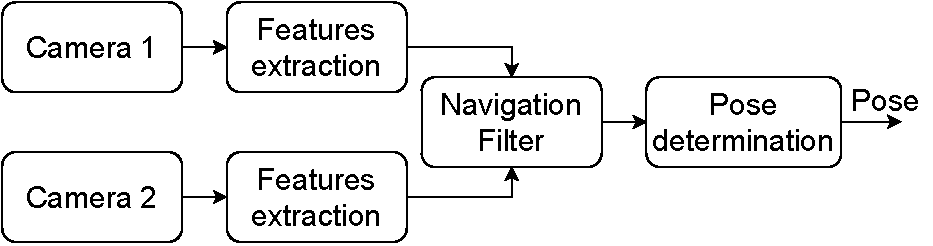
\includegraphics[width=\textwidth]{Images/tight.pdf}
         \caption{Tightly coupled}
         \label{fig:tightc}
     \end{subfigure}
     \hfill
     \begin{subfigure}[b]{0.48\textwidth}
         \centering
         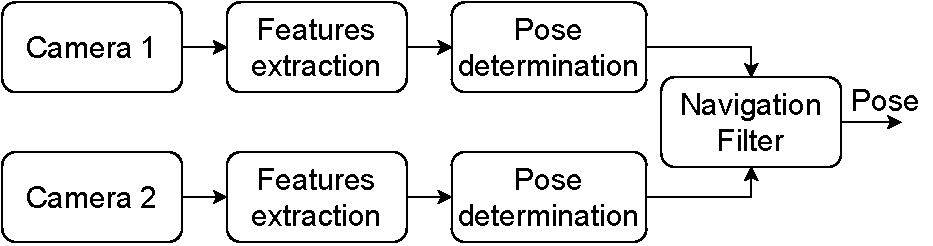
\includegraphics[width=\textwidth]{Images/loose.pdf}
         \caption{Loosely coupled}
         \label{fig:loosec}
     \end{subfigure}
        \caption[Tightly and loosely coupled filters]{Tightly and loosely coupled navigation filter architecture using two cameras}
        \label{fig:filtersheme}
\end{figure}

Loosely coupled are usually preferred for applications where the target is fully known, as the computational time of tightly coupled approaches depends on the number of features detected and they lack robustness to fast relative dynamics \cite{pesce2019autonomous}. However, if the inertia properties of the target are unknown,  tightly coupled filters can retrieve them \cite{volpe2017pose}.\\ 
A very widely used filter in relative navigation applications is the Extended Kalman Filter (EKF) \cite{sharma2017reduced, pesce2019autonomous, galante2016fast} because of their balanced ratio between low complexity and sound performances. As relative dynamics are intrinsically non-linear, the EKF exploits the linearization of the dynamics. In the case of highly non-linear dynamics, non-linear filters are implemented. In the works \cite{volpe2017pose, zhang2015unscented}, the Unscented Kalman Filter is exploited to improve the filter's accuracy, but with the degradation of the computational efficiency. In \cite{pesce2019comparison}, several non-linear filtering techniques such as Minimum Energy Filter, 2nd Order Energy Filter, and Attitude Observer were investigated, uncovering that they outperform linear filters.


\subsection{Multispectral data fusion}
Multispectral navigation is an emerging area of interest for space applications, yet the literature on this topic is still limited. Data fusion can be performed at different levels. The lowest level is to perform image fusion (image-level data fusion), creating from two images in different spectra a composite image with the best characteristics of the two. An extensive survey of methods for image fusion is reported in \cite{singh2021review}. 
In \cite{civardi2022vis}, different methods are applied to the fusion of space imagery performing a comparative assessment. These findings were applied in \cite{bechini2022robust}, where fused images were used to perform pose initialization, demonstrating that fused images can be a reliable source of measurements for navigation algorithms. \\
If the information fusion is performed at a higher level, then the problem can be approached with classical sensor fusion techniques. Odometry fusion techniques are divided into optimization-based, and filter-based techniques \cite{yang2022sensors}. In the former, the state is estimated after processing the measurements acquired into an optimization problem. These methods are more accurate than filter-based methods, although presenting a higher level of complexity \cite{jia2021lvio}. \\
In filter-based approaches, the sensor information is fused inside the navigation filter, as described in \cref{sec:visfilter}. This methodology has been investigated for multispectral sensor fusion in the context of the ESA study "Image Recognition and Processing for Navigation (IRPN)" \cite{sonnenburg2016image}. The interest in this approach was also expressed in \cite{galante2016fast}, fusing VIS, TIR, and LiDAR measurements employing a loosely-coupled Kalman Filter. To the best of the author knowledge, a tightly coupled approach for multispectral data fusion has not been investigated for space applications.\\ 
Further research has been performed in the context of asteroid navigation. In particular, \cite{civardi2021small} uses a loosely coupled approach to fuse multispectral data, while \cite{piccinin2023spacecraft} investigates both a multi-modal approach and image fusion. Both studies focus on a SLAM algorithm, as the map of the asteroid is not known a priori.\\
The lack of literature in the field of multispectral data fusion applied to relative navigation highlights the need for further research in this area, aiming at paving the road for robust navigation pipelines for harsh environments as the one of Active Debris Removal.  

\section{Research objectives and overview}
\chaptermark{Introduction}
The paragraph highlights the thesis scope and its logical flow. It presents the research objectives and formulates them as research questions. The thesis overview and the document structure is presented.


\subsection{Objectives}
The core motivation of the thesis is the enhancement of visual relative navigation techniques about uncooperative targets whose shape is known, given the context explained in \cref{sec:contandmotiv}. In particular, the principal aim of the thesis is: 
\begin{tcolorbox}
\textit{to investigate the potential in exploiting visible and thermal imaging measurements fusion for enhancing relative navigation about known uncooperative space targets.}
\end{tcolorbox}

The thesis aims at providing a deeper understanding of the contribution of multispectral imaging to the estimation of the relative attitude and center of mass position. Specifically, it investigates how sensor fusion expands the range of applicability and increases the performances of monocular visible navigation by combining data from multiple spectra. Moreover, the effectiveness of thermal navigation as a standalone solution is presented, studying the possibility of substituting the visible counterpart when the output of the latter is compromised. In this context, 
the effort is focused on assessing most suitable strategy between privileging either visible or thermal measurements depending on environmental conditions or going straight forward with data fusion always, no matter of external conditions.
%it is studied which is the best solution for multispectral imaging measurements management; aiming at understanding if it is convenient to discard the visible or thermal imaging sensors in certain environmental conditions or if data fusion is always the optimal solution.
The work proposes a solid basis for a comparison with different data fusion techniques, providing further understanding about at which level the multispectral data shall be fused to obtain the most proper results.\\
% To develop the proposed objectives a novel visual navigation chain based on multispectral monocular measurements is proposed and tested. The investigated pipeline focuses on a tightly coupled filtering approach for sensor fusion. The algorithm is \\
Additionally, this work provides valuable insights into best practices and potential pitfalls whenever designing simulation frameworks for testing visual navigation algorithms.\\

\subsection{Research questions}
The thesis objective is then articulated in the following research questions:

\begin{enumerate}
    \item can multispectral imaging improve relative navigation about a known non-cooperative target? What is the contribution of thermal imaging?
    \item Which is the most effective visible and thermal imaging measurements management to improve relative navigation?
    \item Can thermal imaging sensors provide a standalone solution to the relative navigation problem? What are the most prominent limitations of \textit{thermal-only} navigation?
    \item Upon what criteria VIS-IR measurements fusion is preferred against treating them as split inputs?
    Is there an overall winner among the tightly, loosely coupled and image-fusion based approaches?
    %\item At which level is it more convenient to fuse the information of the multispectral sensors? Is a tightly coupled approach better performing that loosely coupled or image-level fusion?
    
\end{enumerate}


\subsection{Thesis overview}
% \section{Intended contribution and thesis outline}
% \chaptermark{Introduction}

To develop the aforementioned objective, this thesis proposes a novel multispectral navigation pipeline for pose tracking with measurements obtained from a VIS and TIR monocular cameras. The algorithm exploits the information extracted from the images to perform model-based pose estimation with respect to the target. The sensor fusion and the pose refinement are performed with an Extended Kalman Filter. The multispectral information is fused at feature level with a tightly coupled approach. In particular, the features tracked on the VIS and TIR images represent the measurements fed into the Kalman Filter, while the pseudo-measurements are computed by projecting the model landmarks onto the image plane. Such fusion technique enables avoidance of the execution of pose reconstruction routines such as the PnP, without the need to expand the filter's state vector, as commonly performed in tightly coupled approaches. In the proposed solution, an online adaptation of the filter's characteristic matrices is employed to tune the contribution of the different features based on the data quality.\\
Although the proposed algorithm's primary goal is to investigate the benefits of combining multispectral imaging sensors, this work is intended to be the basis for a future onboard implementation of the algorithm. For this reason, special attention is given to the computational time required and the complexity of the steps of which the navigation chain is composed.\\
The proposed navigation chain is validated exploiting synthetic images of a space debris. The results are presented and discussed to reach the thesis objective and answer to the research questions.\\
% The proposed architecture is tested to assess its robustness to different conditions and to stress both the visible and the thermal cameras. The same pipeline is also used to investigate the possibility of performing TIR-only navigation in the case of the unavailability of VIS measurements in conditions such as the eclipse.\\
% From these analyses, the thesis aims at providing a deeper understanding of the contribution of multispectral imaging to the relative navigation problem. Specifically, it investigates how sensor fusion expands the range of applicability of monocular visible navigation by combining data from multiple spectra to improve robustness in challenging environments. Moreover, the effectiveness of thermal navigation as a standalone solution is presented, studying the possibility of substituting the visible counterpart when its output is compromised. \\
% Additionally, this work provides valuable insights into best practices and potential pitfalls when designing simulation frameworks for testing visual navigation algorithms.\\
%
%
%
%
%
%  This work investigates a multispectral visual navigation pipeline for pose estimation of a known uncooperative target using a visible and a thermal monocular camera only. 
% The proposed architecture exploits a tightly coupled filtering approach to fuse the data coming from a TIR and a VIS camera. 
% The work focuses on the tracking aspect only, leaving the initial acquisition as a possible future development of the thesis.\\
% The proposed pipeline is composed of an Image Processing (IP) algorithm for extracting and tracking the corner features on the multispectral images and an Adaptive Extended Kalman Filter to fuse the information coming from the two sensors. The filter's state comprises the relative position and attitude of the target, and it exploits as measurements to refine the pose the position of the extracted features on the image. Furthermore, the filter's internal matrices online adaptation results in the contribution of each sensor being contingent on the quality of the data it provides, thereby optimizing each camera's performance under all operational conditions. \\
% The proposed architecture is tested to assess its robustness to different conditions in order to stress both the visible and the thermal camera. The same pipeline is also used to exploit the possibility of performing TIR-only navigation in the case of the unavailability of VIS measurements in conditions such as the eclipse. \\
%This thesis intends to contribute to assessing the performance and robustness of multispectral visual navigation and developing innovative pose estimation schemes to operate in demanding environments. \\
The thesis is structured as follows:
\begin{itemize}
    \item \textbf{Chapter 2} provides a brief explanation of the principles at the basis of the thesis, ranging from aspects of computer vision to preliminary aspects of non-linear estimation methods used. 
    \item \textbf{Chapter 3} presents the proposed visual navigation pipeline, introducing both the filter structure and the IP algorithms used.
    \item \textbf{Chapter 4} describes the simulation framework used to validate the proposed solution to the estimation problem.
    \item \textbf{Chapter 5} presents the simulations' outcome, providing a critical analysis of the obtained results.
    \item \textbf{Chapter 6} summarizes the key findings, identifying the final conclusions. Ideas for future works are also reported.
\end{itemize}
